
The experiment was designed to get a better understanding about the contribution linear and angular velocity, oscillation angle, direction, and orientation can give to the expression of \textit{Happiness}, \textit{Anger}, \textit{Sadness}, and \textit{Fear}, which are four out of the six emotions considered by Ekman~\cite{Ekman2004} as basic emotions, which are characterized to have short duration, cultural universal~\cite{Ekman94}, derive from evolution~\cite{Buck99}, and could influence cognition and action~\cite{Campos2004}. Moreover, these four emotions here selected are overlap with emotion schemas~\cite{Izard2007}.
%%%%%%%%%%%%%%%%%%%
%%%%%%%%%%%%%%%%%%%

\subsection{Independent Variables}

The definitions of the selected independent variables are reported here below.

\begin{itemize}
	\item \textbf{Angular velocity} is the rotational velocity  ($\omega$) of the robot with respect to its center.

	\item \textbf{Oscillation angle} is the maximum extension of the robot's rotation around its center in the oscillating movement ($\theta$).

	\item \textbf{Linear velocity} is the rate of change of the position of the robot ($V$). 

	\item \textbf{Direction with respect to participant's perspective} is the angle generated from the participant's point of view with respect to the robot's trajectory ($D$).

	\item \textbf{Orientation of the body with respect to participant's perspective} is the robot's body orientation with respect to the robot's trajectory ($\phi$).

\end{itemize}

The three first variables are depicted in Figure~\ref{fig:angular_movement}. The robot's frame of reference is drawn to show that it could move straight while it is rotating. It is important to highlight that linear velocity is respected when the robot is also oscillating.


\begin{figure}
	\centering
	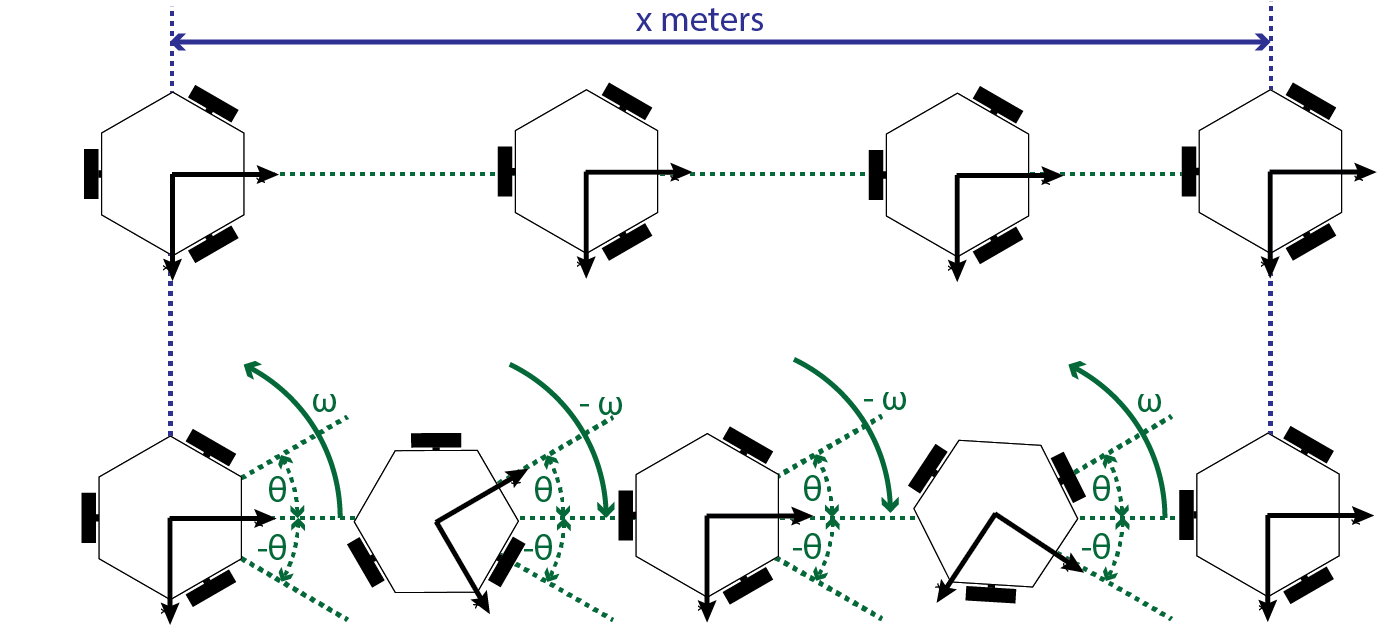
\includegraphics[width=0.48\textwidth]{./Images/ExampleMovement.png} 
	\caption{Example of the features used in the experiment. $x$ represents the displacement in meters, $\omega$ is the angular velocity ($rad/s$) and $\theta$ the oscillation of the body around its center ($rad$). The upper sequence depicts a movement based only on linear velocity, while the bottom one shows a sequence with angular and linear movement. The two black arrows in the robot's middle depict robot's frame of reference.}
	\label{fig:angular_movement}
	
\end{figure} 

\subsubsection*{Independent Variables values}

Specific, discrete values were selected for all independent variables, to make the experiment feasible. First, a simple test to evaluate when significant changes could be perceived was performed on a small sample of independent subjects. Based on this test, specific values for oscillation angle, and angular and linear velocities were selected. The values for the remaining two variables were selected to verify the impact of direction and orientation. This goes in accordance to our observations in previous case studies~\cite{angel2014}, in which people had a better recognition of fear when the robot was moving far. The chosen values are shown in Table~\ref{table:variables_values}. 

\begin{table}[htb]
\centering
\caption{Values for each of the independent variables in the experiment.}
\begin{tabular}{|c|c|c|c|c|}
\hline
\backslashbox{Variable}{Possibilities} & First & Second & Third & Fourth\\
\hline   
Angular Velocity ($rad/sec$)& $0$ & $1$ & $2$ & $3$\\
\hline
Oscillation Angle ($rad$)& $0$ & $0.087$ & $0.175$ & $0.349$\\
\hline
Linear Velocity ($mm/sec$) & $0$ & $200$ & $500$ & $900$\\
\hline
Direction ($rad$)&$0$&$\pi$&$\frac{-\pi}{2}$& \\
\hline
Orientation ($rad$) & $0$ & $\pi$ & & \\
\hline 
\multicolumn{5}{c}{}
\end{tabular} 
\label{table:variables_values}
\end{table}

To get a better idea about the Direction and Orientation values, in Figure~\ref{fig:possibilities_orientation_direction} are reported all  possibilities for these two variables.

\begin{figure}
	\centering
	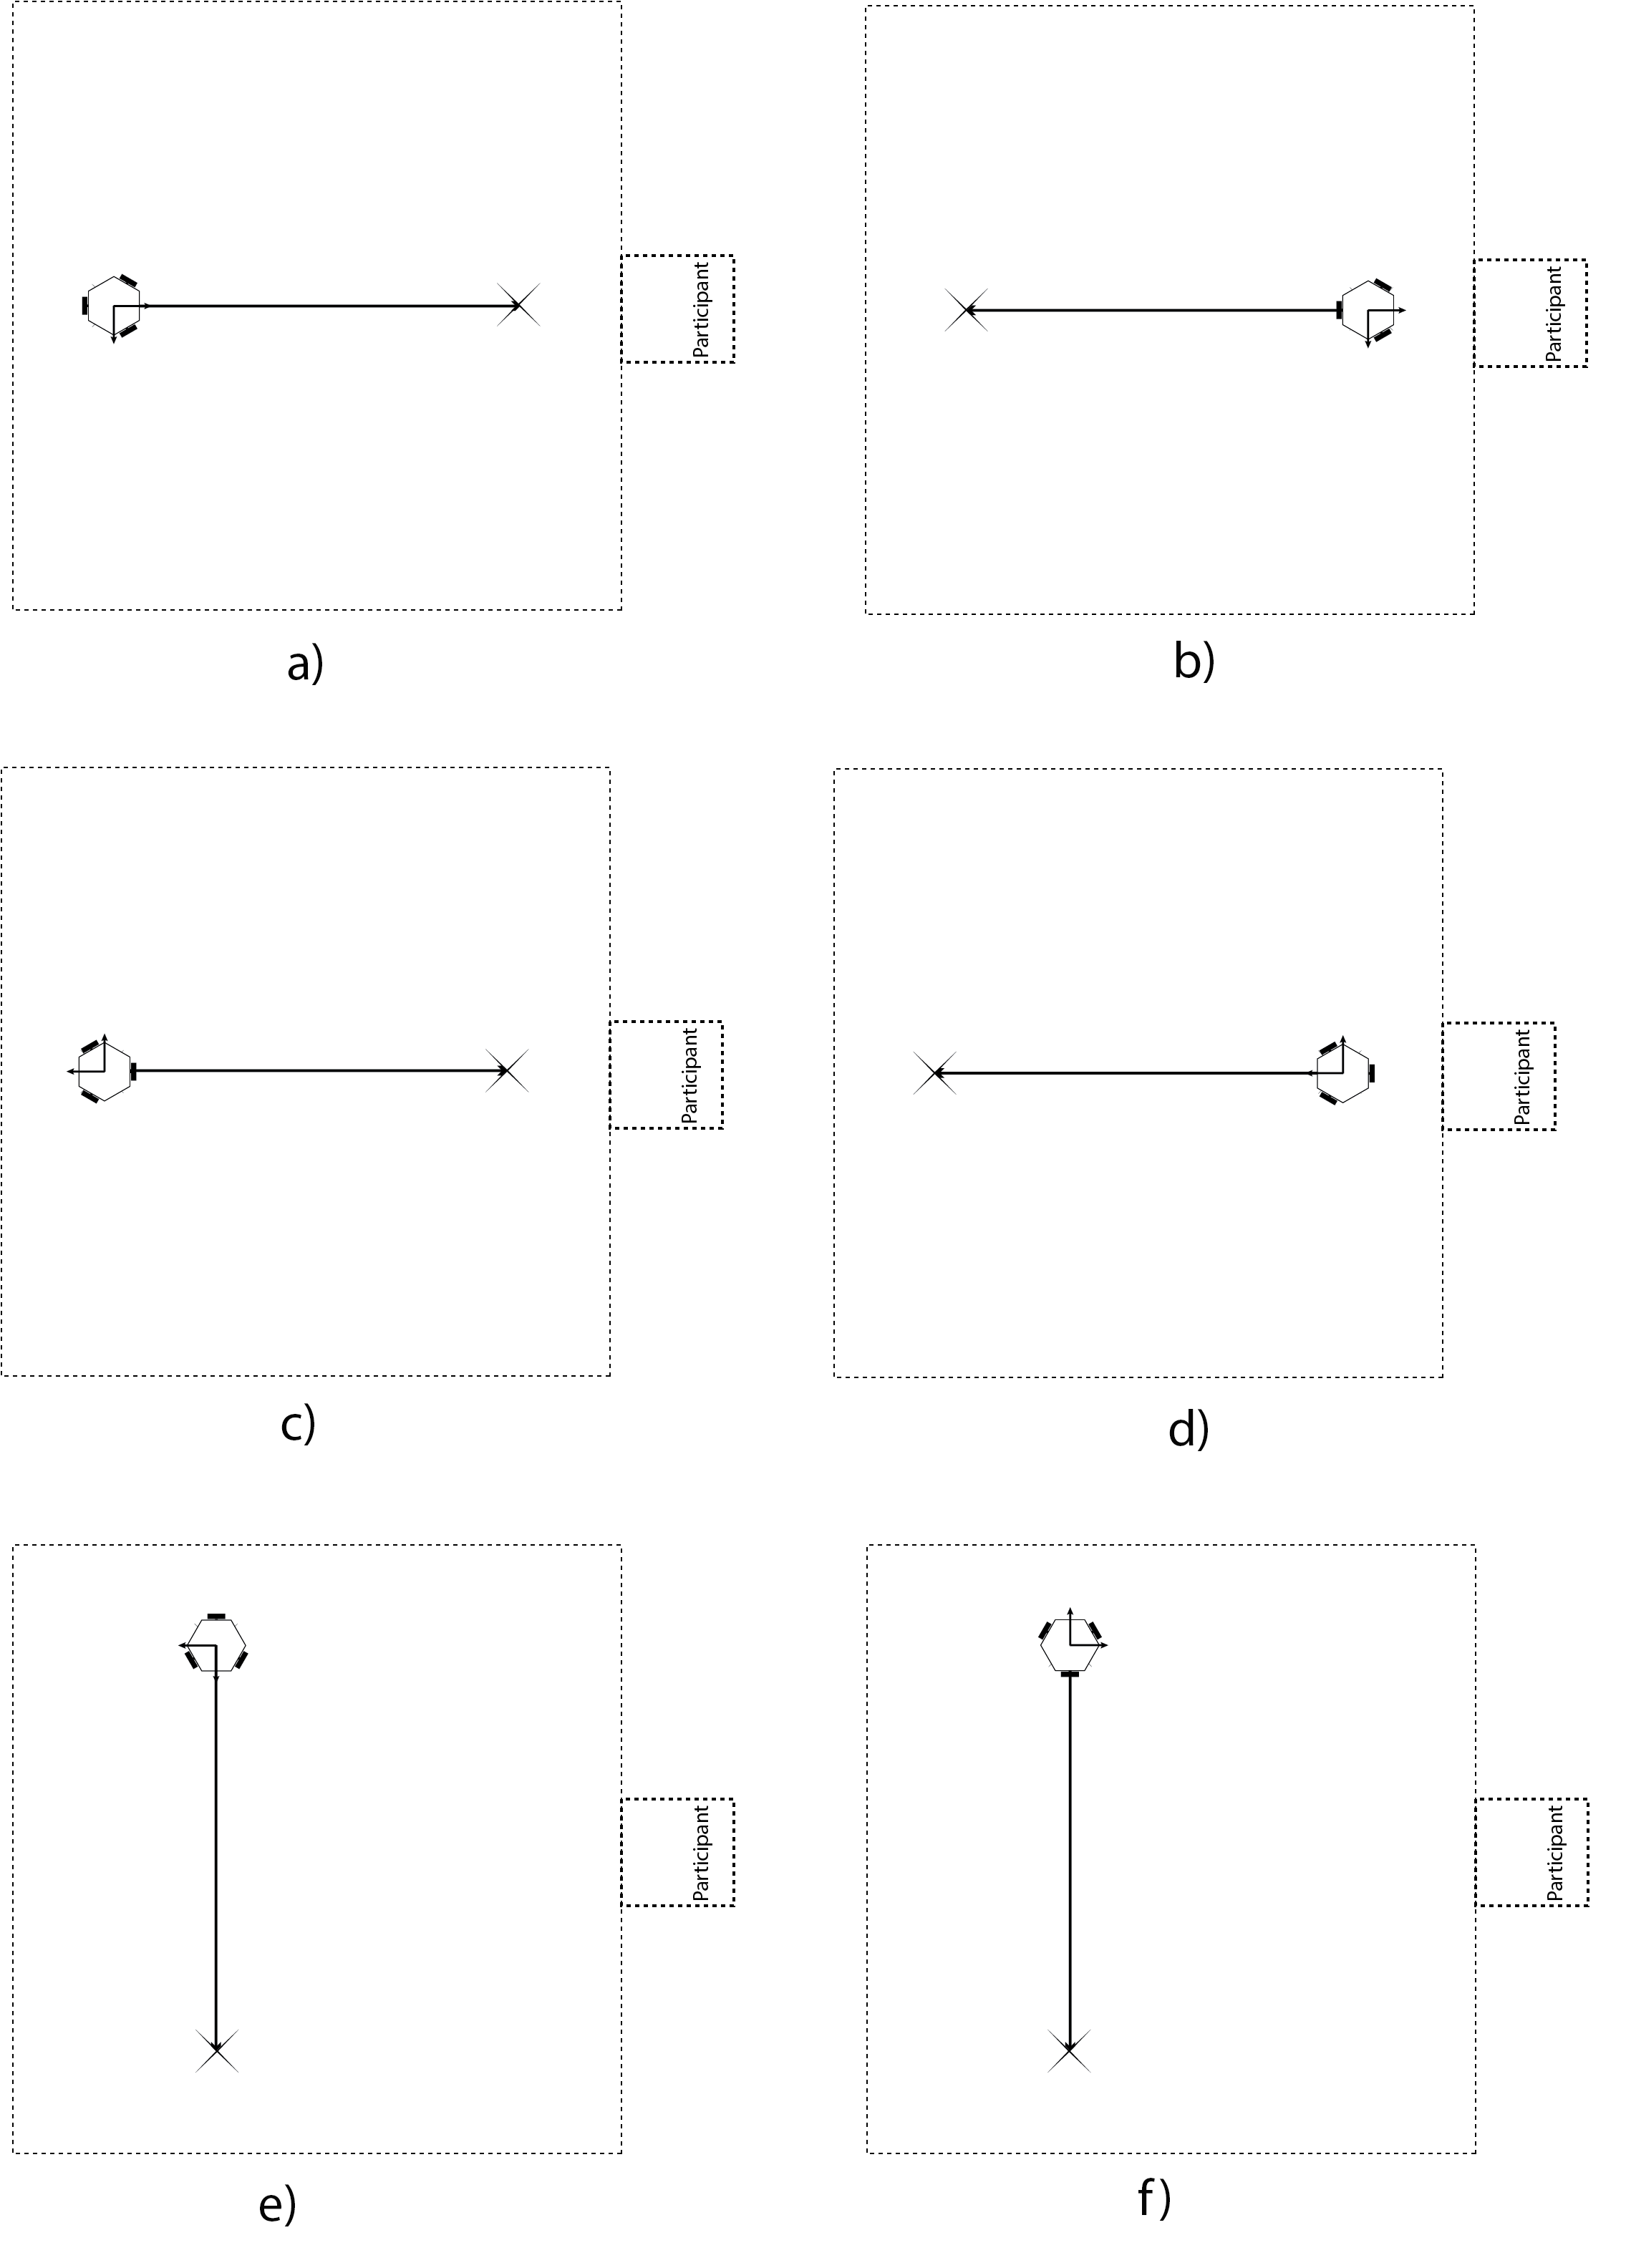
\includegraphics[width=0.48\textwidth]{./Images/possibilities_case.png} 
	\caption{Combination of direction and orientation. The crosses symbolize the final position. The robot represents the initial position with its orientation, which is represented through the robot's frame of reference. The dashed big square represents the robot's movement zone, while the small one on the side represents the subjects' zone. a) Direction = $0$ and Orientation = $0$. b) Direction = $0$ and Orientation = $\pi$. c) Direction = $\pi$ and Orientation = $\pi$. d) Direction = $\pi$ and Orientation = $0$. e) Direction = $\frac{-\pi}{2}$ and Orientation = $0$. f) Direction = $\frac{-\pi}{2}$ and Orientation = $\pi$}
	\label{fig:possibilities_orientation_direction}
\end{figure}

Treatments, meant as desired combination of independent variables to compare~\cite{oehlert2000first},
were generated from the combination of independent variables' values for a total of 384 combinations. Treatments that would not add any significant information to the experiment were removed, such as treatment with $\theta=0$ and $\omega \neq 0$, which reduced total amount of treatments to 195.

%%%%%%%%%%%%%%%%%%%
%%%%%%%%%%%%%%%%%%%
%%%%%%%%%%%%%%%%%%%
\subsection{Dependent Variables}

Two dependent variables were determined, and they are described below.

\begin{itemize}
	\item \textbf{Emotion} is the feeling perceived by the participants from the robot's movement. From previous experiences~\cite{angel2014}
	, it was decided to ask the participants to select an emotion name in a list including the four emotions intended to be expressed, two mental states that could be misinterpreted from these emotions, and the option of ``other''. 
	The two  states of mind included as confounding terms are tenderness and excitement, which correspond to low and high arousal states.
	
	\item \textbf{Emotion's intensity} indicates the emotion intensity as perceived by the subject. This variable is measured on a Likert scale, ranging from 0 to 10, where 0 means that the corresponding emotion is not perceived by the subject and 10 that the emotion is highly perceived by the subject. 

\end{itemize}
%%%%%%%%%%%%%%%%%%%
%%%%%%%%%%%%%%%%%%%

%%%%%%%%%%%%%%%%%%%
\subsection{Participants}

It was decided that each subject had to be exposed to twenty over 195 possible treatments. Each presentation lasted  from 10 to 15 minutes. This was decided because each subject was a volunteer, so the time dedicated to the experiment had to be kept limited. The twenty treatments were selected picking a number without replacement from 1 to 195. A total of 980 answers were collected, guaranteeing a minimum of 5 trials for each treatment. 

The experiment was performed at Politecnico di Milano, involving subjects with different backgrounds.
A total of 49 volunteers were involved: 12 females and 37 males. The average age of the subjects was 25.28, with standard deviation of 2.8, with a minimum age of 20 and maximum of 32. The subjects' country of origin and their backgrounds are shown in the Table~\ref{table:country} and Table~\ref{table:career}, respectively. 

%%%%%%%%%%%%%%%%%%%%% 
\begin{table}[h]
\centering
\caption{Subjects' Country of origin.}
\label{table:country}
\begin{tabular}{|c|c|}
\hline
\textbf{Country} & \textbf{Counting} \\
\hline
Albania & 1 \\
\hline
Bosnia & 1 \\
\hline
Brazil & 2 \\
\hline
Colombia & 4 \\
\hline
Germany & 1 \\
\hline
Greece & 1 \\
\hline
Iran & 5 \\
\hline
Italy & 33 \\
\hline
Moldova & 1 \\
\hline 
\multicolumn{2}{c}{}
\end{tabular} 
\end{table}
%%%%%%%%%%%%%%%%

\begin{table}[h]
\centering
\caption{Subjects' Background.}
\label{table:career}
\begin{tabular}{|c|c|}
\hline
\textbf{Career} & \textbf{Counting}\\
\hline
Aeronautical Engineering & 1 \\
\hline
Architecture & 1 \\
\hline
Social assistance & 1 \\
\hline
Automation & 1 \\
\hline
Bio-medical Engineering & 5 \\
\hline
Computer Science & 33 \\
\hline
Electronic Engineering & 2 \\
\hline
Mechanical Engineering & 2 \\
\hline
Nursery & 1 \\
\hline
Pedagogical Science & 1 \\
\hline
Tourism & 1 \\
\hline
\multicolumn{2}{c}{}
\end{tabular} 
\end{table}
%%%%%%%%%%%%%%%%%%%

The information from each subject was collected using a web-based form. To maintain anonymity, no personal information that could be used to trace the subject back was collected. The procedure used with each subject is described here below.

\begin{enumerate}
	
	\item The subject was asked to fill out the following information:
	
	\begin{itemize}
		\item Sex
		\item Background
		\item Age
		\item Country of origin
	\end{itemize}
	
	\item The robot was shown to the participant and the experiment procedure explained.

	\item An example of the questionnaire was presented and a sample movement of the robot shown.

	\item The subject was exposed to a specific movement sequence according to the following steps:

	\begin{enumerate}

		\item The subject is exposed to the movement generated by a configuration of values.

		\item The subject could use as much time as needed to select values for intensity of the different terms in the questionnaire.

		\item After the subject had completed his/her selection about the current movement, the robot is positioned to the new starting point, and the sequence is repeated from step 1.(a) for the rest of movements.

	\end{enumerate}
\end{enumerate}

The order of the options listed in the questionnaire changed for each question to prevent any kind of bias. Figure~\ref{fig:questionnaire_example} shows an example of the questionnaire used. 

\begin{figure}
	\centering
	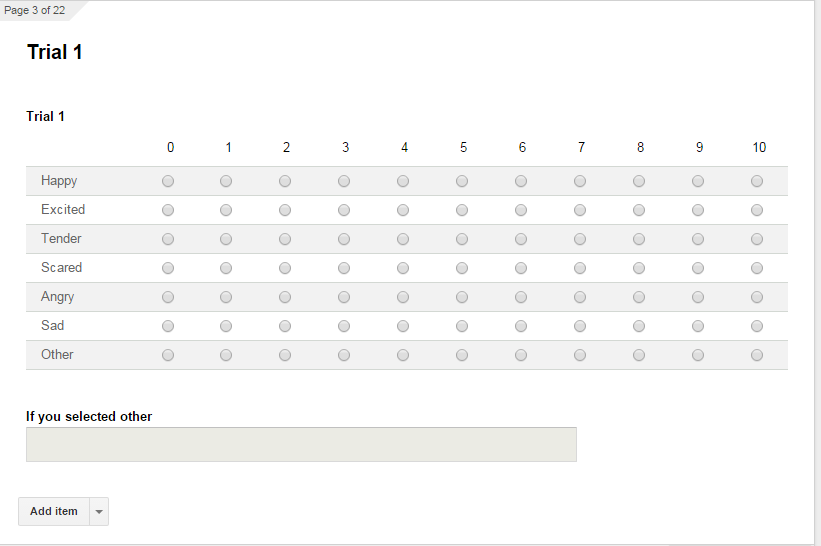
\includegraphics[width=0.48\textwidth]{./Images/example_survey.png} 
	\caption{Example of the questionnaire used in the experiment.}
	\label{fig:questionnaire_example}
\end{figure}

\subsection{Setup}

The experimental setup and dimensions are shown in the Figure~\ref{fig:setup}. The crosses symbolize possible starting points, which were selected depending on the direction's value, as it is showed in Figure~\ref{fig:possibilities_orientation_direction}. 

\begin{figure}
	\centering
	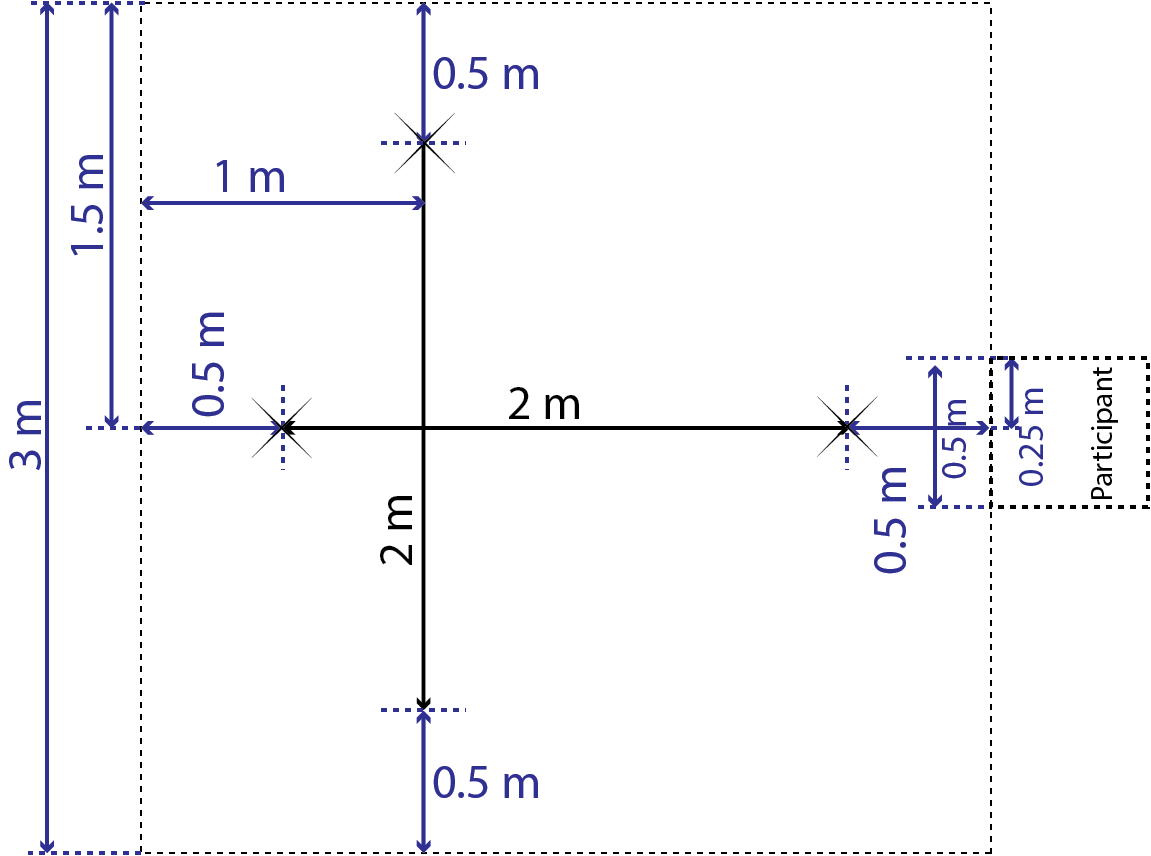
\includegraphics[width=0.45\textwidth]{./Images/ExperimentGeneral.png} 
	\caption{Setup for the experiment. The crosses symbolize the possible starting points.}
	\label{fig:setup}
\end{figure} 